
\section{Implementação do Padrão de Visitante (\texttt{walker})}

Desenvolvemos o pacote \texttt{walker} para auxiliar em 3 tarefas chaves: validação de precedencia da AST gerada pelo \textit{parser}; visualização da AST gráficamente; geração de código. O padrão visitante foi empregado para percorrer e operar em uma AST. Uma estrututa e uma função implementam esse padrão e agem em cima da AST. procedimentos implementam esse padrão e manipulam a AST: \texttt{Visitor} e \texttt{walk}, respectivamente.


O padrão visitor implementado na função \texttt{walk} representa um mecanismo genérico e recursivo para travessia da AST, permitindo a aplicação de transformações ou análises personalizadas em cada nó da árvore.

A estrutura \texttt{Visitor} (\autoref{cod-visitor-struct}) encapsula uma função de visita polimórfica que pode ser chamada para cada tipo de nó, possibilitando um processamento flexível e extensível, onde o visitante pode modificar seu próprio estado durante a travessia, decidir continuar ou interromper o caminhamento, e realizar operações arbitrárias como transformação, análise semântica, geração de código ou depuração.

A função, no \autoref{cod-visitor-walk} implementa uma travessia profunda (\textit{depth-first}) recursiva, que automaticamente percorre todos os nós da AST, incluindo declarações, expressões, statements e estruturas aninhadas, invocando a função de visita antes e depois da exploração de cada subárvore. Isso é utils para criação de visitors personalizados para diferentes propósitos como checagem de tipos, parentização de expressões, geração de gráficos para arvóre.


\begin{codigo}[htb]
    \caption{\small Estrutura polimórfica \texttt{Visitor}}
        \label{cod-visitor-struct}
\begin{lstlisting}[language = C]

// Estrutura polimórfica, aceita um tipo qualquer, chamado de DataType, como estrada para criar um tipo concreto.
Visitor :: struct (DataType: typeid) {
    visit: proc(visitor: ^Visitor(DataType), node: ^ast.Node) -> ^Visitor(DataType),
    data:  DataType,
}
\end{lstlisting}
\end{codigo}

\begin{codigo}[tb]
\caption{\small Estrutura \texttt{Visitor} e função de percurso \texttt{walk}. }
        \label{cod-visitor-walk}
\begin{lstlisting}[language = C]
// Por brevidade vamos omitir varios casos do `switch` que seguem a mesma lógica
walk :: proc(v: ^Visitor($T), node: ^ast.Node) {
    if v == nil || node == nil {
        return
    }
    v := v->visit(node)
    if v == nil {
        return
    }
    using ast
    switch n in &node.derived {
        case ^Start:
            for d in n.decls {
                walk(v, d)
            }

        case ^Decl_Equation:
            walk(v, n.field)

        case ^Field:
            walk(v, n.name)
            walk(v, n.value)

        case ^Expr_Number:     // Caso base

        case ^Expr_Vector_Literal:
            for number in n.numbers {
                walk(v, number)
            }
        case ^Expr_Identifier:
                walk(v, n.sub_expression)

        // ...
        // casos OMITIDOS aqui Também
        // ...
        case ^Expr_Infix:
            walk(v, n.left)
            walk(v, n.right)

        case ^Expr_Grouped:
            walk(v, n.expr)

        case ^Expr_Function_Call:
            walk(v, n.left)
            for e in n.exprs {
                walk(v,  e)
            }
        case:
            assert(false, "Unhandled token on walk_print ")
    }
    v = v->visit(nil)
}

  \end{lstlisting}
\end{codigo}


\subsection{Validação de Precedencia}
Utilizamos o pacote \texttt{walker} para validão precendencia de operadores na AST gerada pelo \texttt{parser}. A função de parentização implementa inserção automática de parênteses que captura a precedência original das operações na AST, garantindo que a representação textual preserve a ordem de avaliação das expressões matemáticas. Através de uma travessia disponivel pelo pacote usado, o algoritmo cria uma cadeia de caraceters com parênteses adicionais em expressões com prefixo, expressões binárias, chamada de funções. Isso é feita todas as os tipos de expressões. 
Essa reprodução explicita da hierarquia de operações permite verificar automaticamente se a construção da AST durante o parsing manteve corretamente as regras de precedência.

Cada teste de precendecia consiste em um texto original e um testo com parenteses esperaros, como demonstrado na listagem \autoref{cod-test-paren}. Tentamos testar os casos mais complexos de expressões matemáticas, operações como exponenciação, que é associativo pela direitoa, combinado com operadores associativo pela esquerda  com diferentes precedencias

À medida que o compialdor foi sendo desenvolvido esses testes se mostraram uteis em previnir quebra do de casos anteriores, pois ao dar suporte a nova funcionalidade, é possivel quebrar funcionalidade já estabelicidade anterioromente.

\begin{itemize}
  \item \textbf{walker\_interp}: interpreta a AST, calculando o valor numérico das expressões.
  \item \textbf{walker\_paren}:   \item \textbf{walker\_print}: imprime os nós da AST e seus atributos, facilitando a depuração e compreensão da estrutura da AST.
\end{itemize}

\begin{codigo}[htb]
    \caption{\small Validação de precendencia por parentização de expressões. }
        \label{cod-test-paren}
  \begin{lstlisting}[language = C]
    test_paren(
        "a = 1+2", // Entrada
        "a=(1+2)"  // Saída Esperada
    );

    test_paren(
        "a = \exp 1 + 2^3", // Entrada
        "a=(\exp(1)+(2^3))" // Saída Esperada
    );

    // ...
    // Outros Testes
    // ...

    test_paren(
        "a = a(1*2 ^ 4 +  \sqrt 4^8 , 2)", // Entrada
        "a=a(((1*(2^4))+(\sqrt(4)^8)),2)"  // Saída Esperada
    );
  \end{lstlisting}
\end{codigo}



\subsection{Visualização da AST por Imagem}

Para validação visual, foi implementado um função que gera uma imagem no formato ``SVG``, que é um formato textual, da arvore contendo informação circulos, representados nós da AST, jutamente com textos subinscritos informados metadados sobre os nós, como o tipo de operador, o tipo de nó, a string do indetificador  no caso de ser @etc.

Como exemplo, na \autoref{fig-svg} temos a visualização do SVG gerado pela equação \autoref{eq-svg}. Notamos que os nós de expressões binárias \texttt{+} e \texttt{-} próximo da raiz seriam avaliados depois, já os nós mais próximo das folhas deve ser resolvidos primeiros indicando um precedencia maior, como expressões binárias \texttt{*} e \texttt{\^}. Esse SVG também anota o tipo da expressão, note que a identificador $f$ é do tipo $\mathbb{R}$), é feito na estapa de \texttt{checker}, veremos mais a frente como isso é feito.
 

@@@
Os nós são heterogeneos, a maneira de acessar um filho de cada nós depende do tipo, pois o campo varia de nome ou posição na es trutura, o pacote walker também permite extrair nós filhos de maneira uniforme para qualquer tipo de nó através de uma função chamada children (\autoref{cod-childre-signature}).(funções como ``children`` que dado um nó abstrato, ele resolve qual o tipo resolvido e cria um array de nós, como extrair os filho). Ela é usada para simplificar o código de geração do SVG ao agir em cima de um nó de maneira uniforme, sem se preocupar com o tipo do nó.

\begin{equation} \label{eq-svg}
   f =  1*2 ^ 4 +  \sqrt 4^8
\end{equation}


\begin{codigo}[htb]
        \caption{\small Assinatura da função que extrai nós filhos de maniera uniforme para qualquer tipo de nó. }
        \label{cod-childre-signature}
  \begin{lstlisting}[language = C]
    // Aceita um ponteiro de nós abstrato e return uma lista de nós filhos
    children :: proc(node: ^Node) -> (array :[dynamic]^Node);
  \end{lstlisting}
\end{codigo}

% \begin{figure}[H]
\begin{figure}[h]
    \caption{\label{fig-svg} \small SVG da AST gerado para \autoref{eq-svg}.}
    \begin{center}
        % 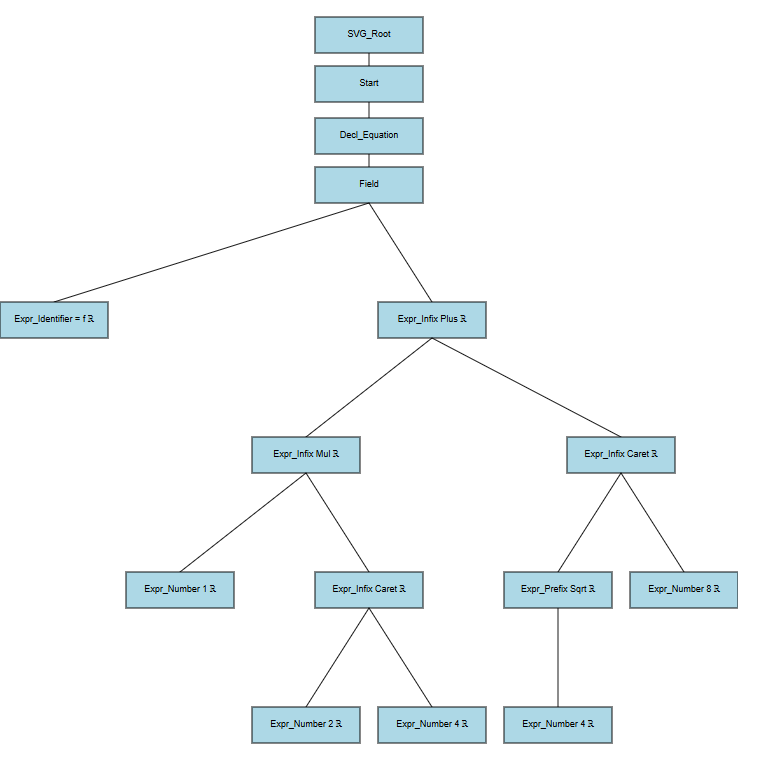
\includegraphics[width=\textwidth, scale=1.1]{./Imagens/svg.png}
        % 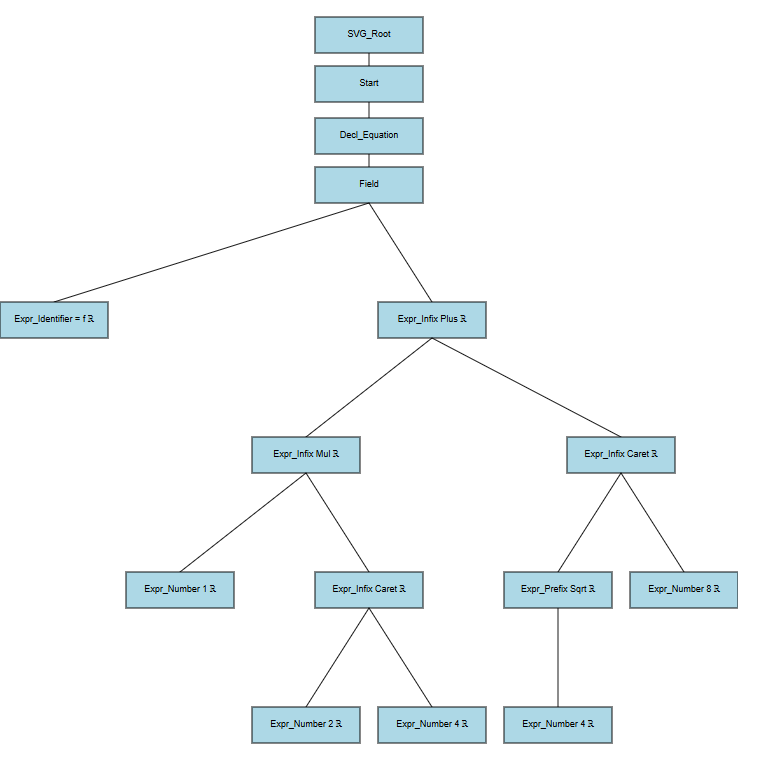
\includegraphics[scale=0.9]{./Imagens/svg.png}
        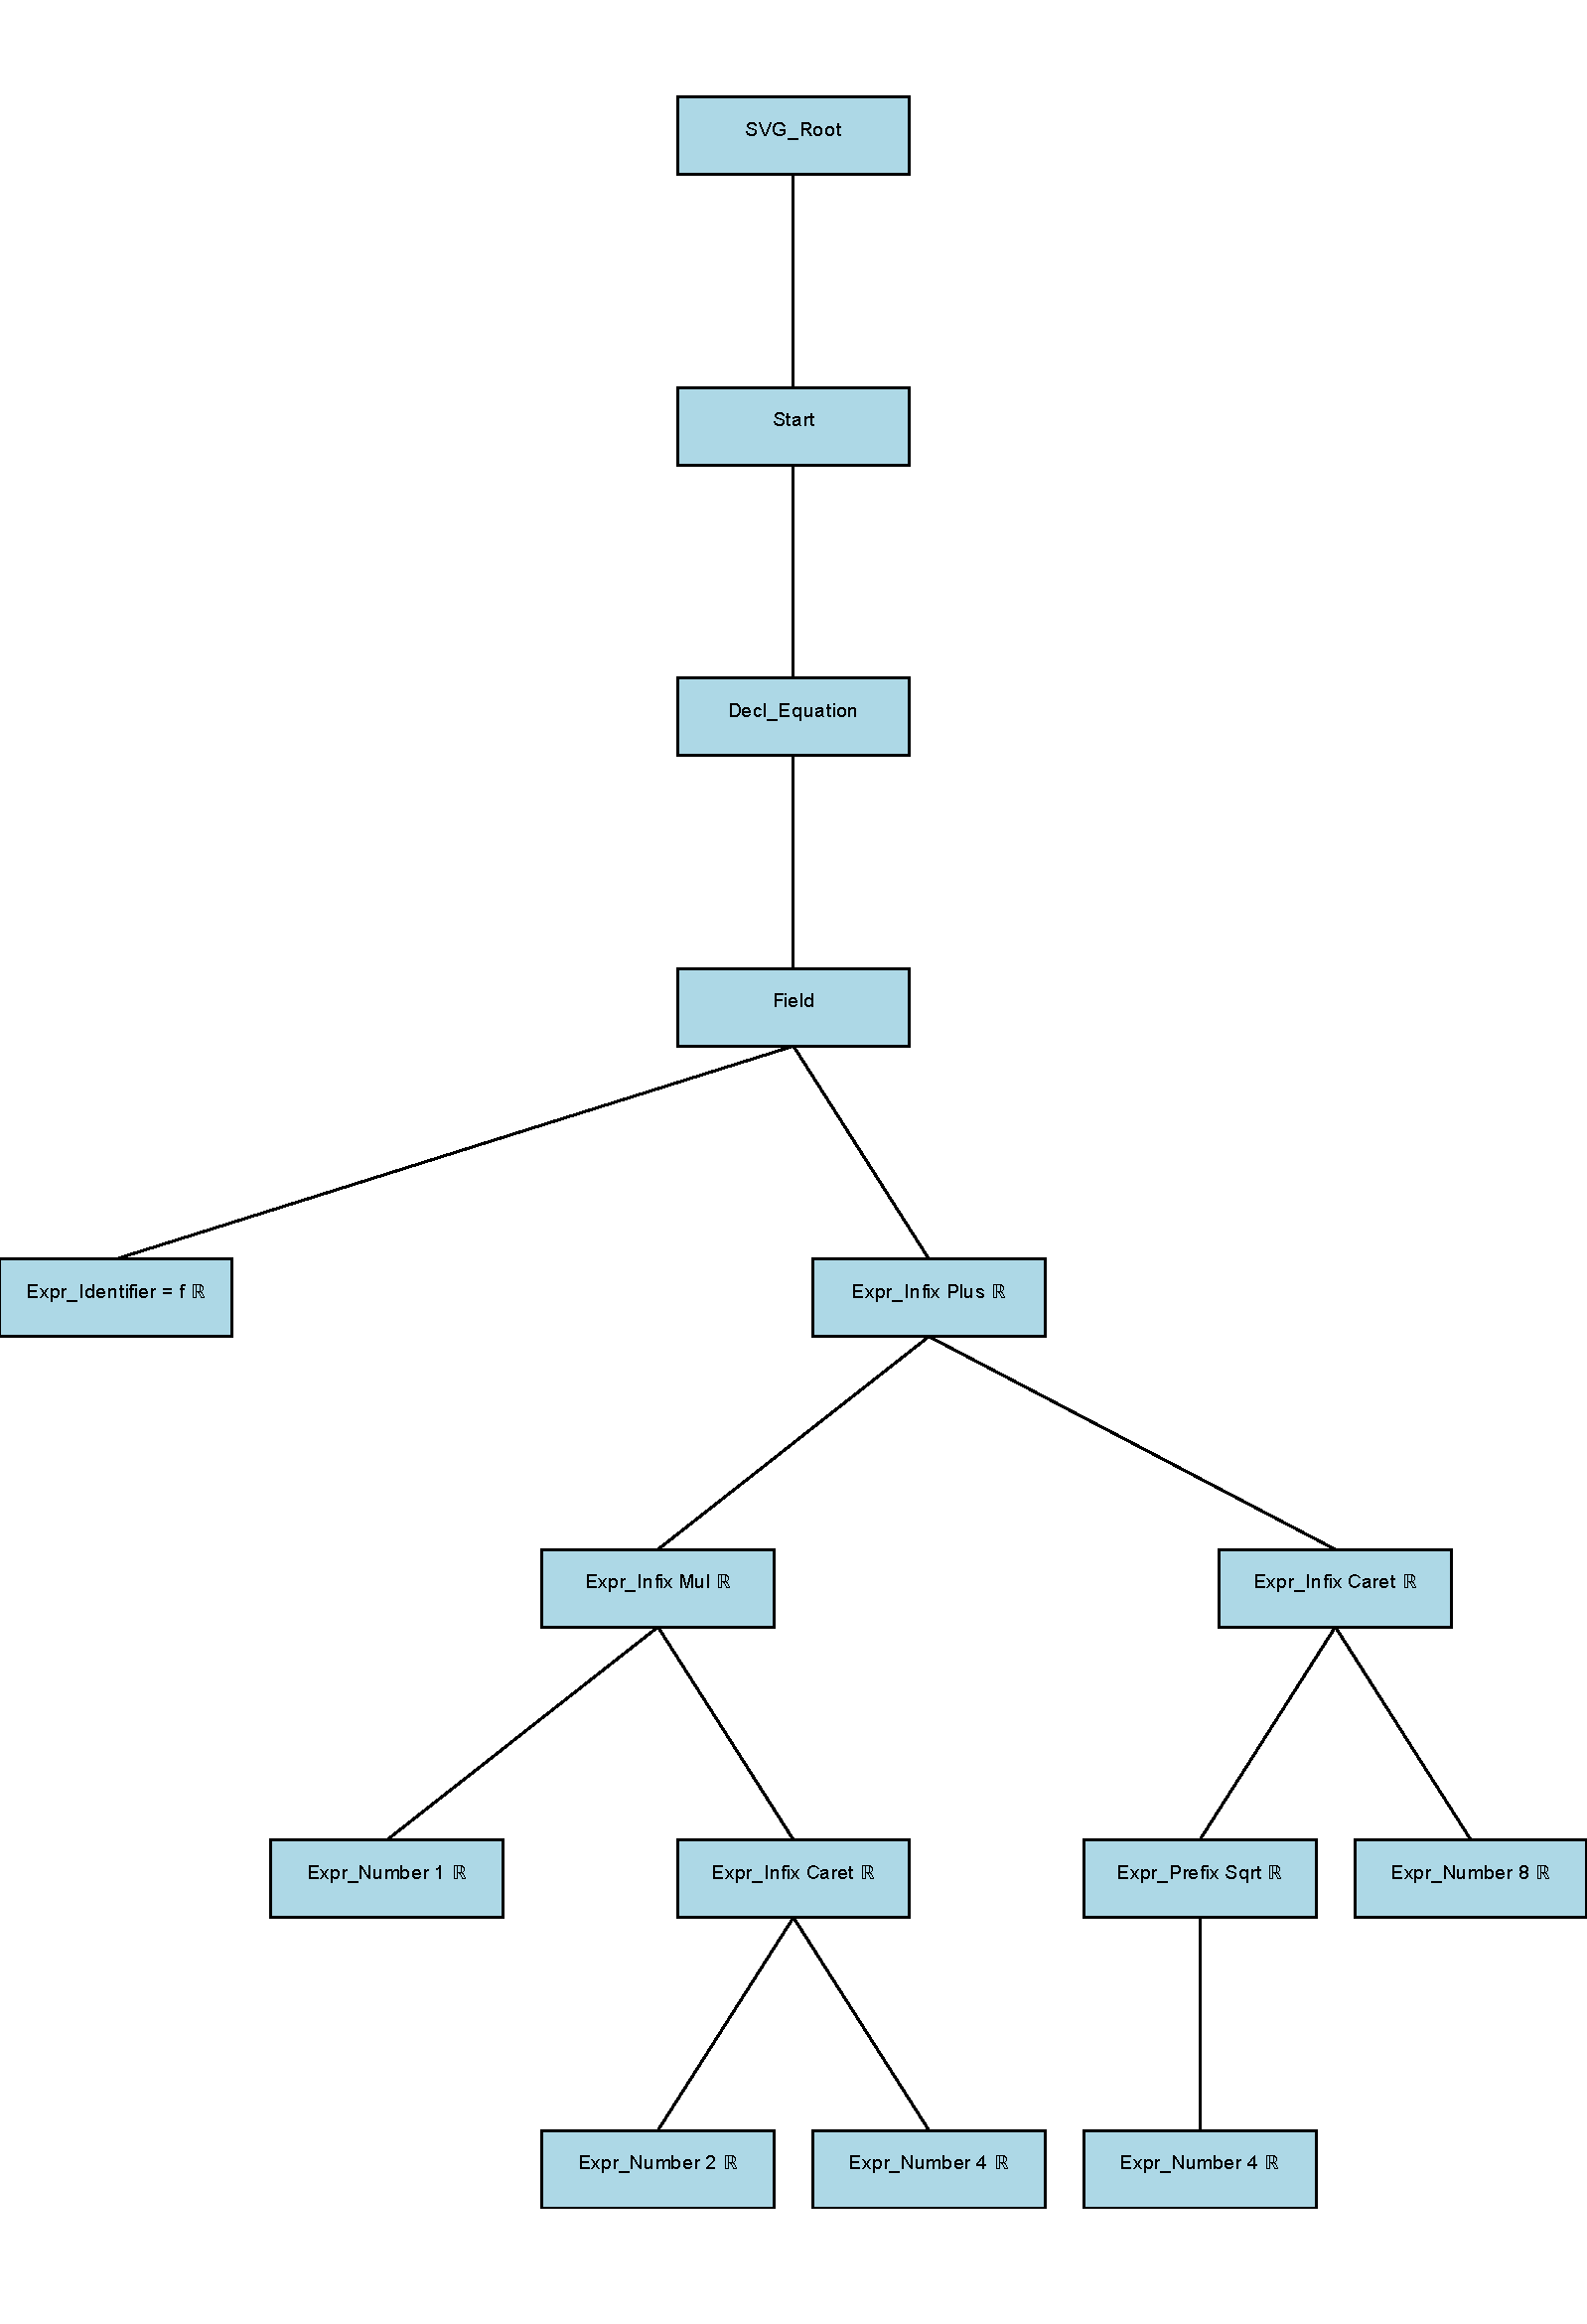
\includegraphics[scale=0.65]{./Imagens/svg.pdf} % Best outta of them all, because it gets to indefinitely zoom in
        % \includesvg[scale=0.9]{./Imagens/svg.svg}
    \end{center}
\end{figure}



% Temos dois tipos de validação dessa precendencia para garantir corretude de implementação de Pratt Parser, uma visual e outra automatica.
% Como mostrado em \autoref{tab-token-precedence} usamos uma tabela para definir a priopridade de operadores,
%
%
% ```
% \begin{equation}
% opertattions ungrouped
%
% \end{equation}
% ```
% Já se agruparmos certas operações, temos e o SVG gerado é diferente mostrando mostrando-se util em auxiliar o desenvolvimento.
%
%
% ```
% \begin{equation}
% grouped
% \end{equation}
% ```
% A maneira automatica é feita utilizando tested que gerandados sobre os casos, cada caso tem um entrada dada e saida esperada. A entrada é uma equação em string, a saída é uma string com a mesma, mas com a ordem de operação explicitamente citada através de parensentese. à Medida que o compialdor foi sendo desenvolvido mais teste foram adicionado para previnir quebra do código a medida que o projeto foi avançando. Alguns exemplos se encontram em @@@ e a informação gerada após aplicar o texto esta em @@@. Adicionamos o parentese através de um outro modulo chamado ``walker``, nele temos acesso à funções como ``children`` que dado um nó abstrato, ele resolve qual o tipo resolvido e cria um array de nós, como extrair os filho de nós heterogeneos precisa ser abstraido, cada estruttura tem campos diferetnes como filho. Outra facilidade que esse pacote desenvolvido é o padrão visitador @@ pegar o padrão visitador que tem função que utiliza generics.
%
%
% ```odin
% SVG_Node :: struct{
%     name: string,
%     children: [dynamic]^SVG_Node,
% };
% ```
% Como mostrado em @@@ usamos uma tabela para definir a priopridade de operadores
% Criamos um tabela que define e atráves de uma função, podemos acessar esses valores
% dado um token temos o reusltado
% Temos dois tipos de validação dessa precendencia para garantir correture de implementação de Pratt Parser, uma visual e outra automatica.
% Para validação visual, foi implementado um função que gera uma imagem no formato ``svg`` da arvore contendo informação circulos, representados nós da AST, jutamente com textos subinscritos informados metadados sobre os nós, como o tipo de operador, o tipo de nó, a string do indetificador  no caso de ser @etc
% Os nós próximo da raiz seriam implementados depois, já os proximos das folhas deve ser resolvikdos pprimeiros indicando um precedencia maior por exemplo
%
% Compilado para gerar a AST em SVG da equação @@, esperamos que '^' ocorra antes '*' que ocorra antes. Ao observar a arvore, notamos que o nó correspondente àoperação '^' ocorre.
%
% ```
% \begin{equation}
% opertattions ungrouped
%
% \end{equation}
% ```
% Já se agruparmos certas operações, temos e o SVG gerado é diferente mostrando mostrando-se util em auxiliar o desenvolvimento.
%
%
% ```
% \begin{equation}
% grouped
% \end{equation}
% ```
% A maneira automatica é feita utilizando tested que gerandados sobre os casos, cada caso tem um entrada dada e saida esperada. A entrada é uma equação em string, a saída é uma string com a mesma, mas com a ordem de operação explicitamente citada através de parensentese. à Medida que o compialdor foi sendo desenvolvido mais teste foram adicionado para previnir quebra do código a medida que o projeto foi avançando. Alguns exemplos se encontram em @@@ e a informação gerada após aplicar o texto esta em @@@. Adicionamos o parentese através de um outro modulo chamado ``walker``, nele temos acesso à funções como ``children`` que dado um nó abstrato, ele resolve qual o tipo resolvido e cria um array de nós, como extrair os filho de nós heterogeneos precisa ser abstraido, cada estruttura tem campos diferetnes como filho. Outra facilidade que esse pacote desenvolvido é o padrão visitador @@ pegar o padrão visitador que tem função que utiliza generics.
%
%
% ```odin
% SVG_Node :: struct{
%     name: string,
%     children: [dynamic]^SVG_Node,
% };
% ```
%
%
% \subsection{Testes}
%
%
% Foi desenvolvida uma série de testes que  abrangem vários aspectos da funcionalidade do \textit{parser}, incluindo geração de árvore de sintaxe, precedência de operadores e interpretação semântica.
%
%
% \subsubsection{Geração de Árvore de Sintaxe}
%
%
% Um aspecto crucial dos testes envolve verificar a correta geração de árvores sintáticas a partir de expressões de entrada. Os testes são projetados para cobrir diferentes cenários, incluindo operações aritméticas simples, expressões complexas com sub-expressões aninhadas e chamadas de funções. São eles:
%
%
% \begin{itemize}
%     \item O manuseio correto de operadores unários e binários, garantindo a precedência e associatividade adequadas.
%     \item A representação precisa de chamadas de função e seus argumentos dentro da árvore de sintaxe.
%     \item O agrupamento adequado de expressões dentro de parênteses para confirmar regras de precedência.
% \end{itemize}
